\documentclass{beamer}
\usetheme{Singapore} 
\setbeamercovered{transparent}
\setbeamertemplate{enumerate subitem}{(\alph{enumii})}
\usecolortheme{rose} 
\useinnertheme[shadow]{rounded}
\usepackage{tikz}
\usepackage{amssymb}
\usepackage{amsthm}
\usepackage{amsmath}
\usepackage{mathabx}
\usepackage{listings}
\usepackage{bbm}
\usepackage{caption}
\usepackage{natbib}
\usepackage{float}
\usepackage{hyperref}
\usepackage{animate}
\usetikzlibrary{patterns,automata,positioning,arrows}
\mode<presentation>
\title{Incentive Compatibility of Multi-Class Logistic Regression}
\author{Young Wu}
\date{\today}
\hbadness=99999

\begin{document}
\newtheorem{thm}{Theorem}
\newtheorem{cor}{Corollary}
\newtheorem{lem}{Lemma}
\newtheorem{prop}{Proposition}
\newtheorem{conj}{Conjecture}
\newtheorem{algo}{Algorithm}
\newtheorem{obs}{Observation}
\newtheorem{clm}{Claim}
\theoremstyle{definition}
\newtheorem{df}{Definition}
\newtheorem{eg}{Example}
\newtheorem{asm}{Assumption}
\newtheorem{cond}{Condition}
\theoremstyle{remark}
\newtheorem{rmk}{Remark}
\begin{frame} \titlepage \end{frame}


\section{Introduction} \subsection{Main}

\begin{frame} \frametitle{Model Setup}
\begin{itemize}
\item There are $n $ agents. Agent $i $ has public $x_{i}$ and private $y_{i.}$
\item The principal uses a publicly known classifier.
\item Agent $i $ chooses to report some $y^{\dagger}_{i}$ to maximize the probability that the classifier classifies $x_{i}$ correctly.
\item Question: for which classifiers, the agents do not have the incentive to misreport their $y_{i}$
\end{itemize}
\end{frame}

\begin{frame} \frametitle{Incentive Compatibility}
\begin{itemize}
\item A dataset is incentive compatible (IC) given a classifier $w^\star $ if there is an $i $ and some $y^{\dagger}_{i} \neq  y_{i}$ such that,
\end{itemize}\begin{align*}
\mathbb{P}\left\{Y = y_{i} | x_{i} ; w^\star \right\} &< \mathbb{P}\left\{Y = y_{i} | x_{i} ; w^\star \left(y^{\dagger}_{i}\right)\right\}.
\end{align*}
\begin{itemize}
\item A classifier is incentive-compatible if all datasets are incentive-compatible given this classifier.
\end{itemize}
\end{frame}



\section{Logistic Regression} \subsection{Main}

\begin{frame} \frametitle{Logistic Regression Example}
\begin{itemize}
\item One numerical example dataset is not incentive-compatible,
\end{itemize}\begin{align*}
\mathbb{P}\left\{Y = \text{\;red\;} | x_{\text{\;square\;}} ; w^\star \right\} &= 0.3290, \text{\;but\;}
\\ \mathbb{P}\left\{Y = \text{\;red\;} | x_{\text{\;square\;}} ; w^\star \left(y^{\dagger}_{\text{\;square\;}} = \text{\;blue\;}\right)\right\} &= 0.4966.
\end{align*}
\begin{figure}[H] \centering 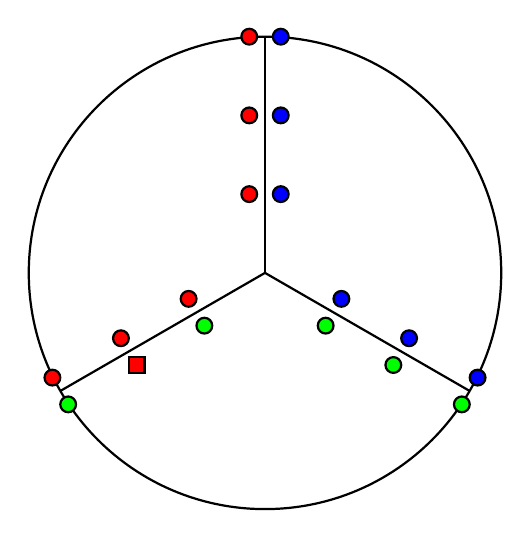
\begin{tikzpicture} [scale = 1] 
\draw[thick] (0.0, 0.0) circle [radius = 3.0];
\draw[thick] (0.0, 0.0) -- (0.0, 3.0);
\draw[fill = blue, thick] (0.2, 1.0) circle [radius = 0.1];
\draw[fill = blue, thick] (0.2, 2.0) circle [radius = 0.1];
\draw[fill = blue, thick] (0.2, 3.0) circle [radius = 0.1];
\draw[fill = red, thick] (-0.2, 1.0) circle [radius = 0.1];
\draw[fill = red, thick] (-0.2, 2.0) circle [radius = 0.1];
\draw[fill = red, thick] (-0.2, 3.0) circle [radius = 0.1];
\draw[thick] (0.0, 0.0) -- (2.6, -1.5);
\draw[fill = blue, thick] (0.97, -0.33) circle [radius = 0.1];
\draw[fill = blue, thick] (1.83, -0.83) circle [radius = 0.1];
\draw[fill = blue, thick] (2.7, -1.33) circle [radius = 0.1];
\draw[fill = green, thick] (0.77, -0.67) circle [radius = 0.1];
\draw[fill = green, thick] (1.63, -1.17) circle [radius = 0.1];
\draw[fill = green, thick] (2.5, -1.67) circle [radius = 0.1];
\draw[thick] (0.0, 0.0) -- (-2.6, -1.5);
\draw[fill = red, thick] (-0.97, -0.33) circle [radius = 0.1];
\draw[fill = red, thick] (-1.83, -0.83) circle [radius = 0.1];
\draw[fill = red, thick] (-2.7, -1.33) circle [radius = 0.1];
\draw[fill = green, thick] (-0.77, -0.67) circle [radius = 0.1];
\draw[fill = red, thick] (-1.73, -1.27) rectangle (-1.53, -1.07);
\draw[fill = green, thick] (-2.5, -1.67) circle [radius = 0.1];
\end{tikzpicture} 
\end{figure}
\end{frame}

\begin{frame} \frametitle{Logistic Regression Experiments}
\begin{itemize}
\item R nnet package is used to estimate the logistic regression coefficients on $10000$ datasets of $100$ iid standard normally distributed points. If the labels are assigned at random, none of the datasets is incentive incompatible. If the random weights are used to create the labels (but with some error), then among the $10000$ datasets:
\end{itemize}
\begin{enumerate}
\item $99952$ are IC
\item $48$ are not IC
\item $7$ are not IC for two or more agents
\item for $4$ datasets from the $48$, after one agent misreports, at least one other agent has the incentive to also misreport as a "defense"
\end{enumerate}

\end{frame}



\section{Other Classifiers} \subsection{Main}

\begin{frame} \frametitle{IC ERM Classifiers}
\begin{enumerate}
\item Binary classifiers (Proposition $2$, requires a technical condition on a loss function. The condition is satisfied for the standard logistic regression)
\item ERM with zero-one loss (Proposition $1$)
\item ERM with $L_{1}$ loss (Dekel, Fischer, Procaccia $2010$)
\end{enumerate}

\end{frame}

\begin{frame} \frametitle{IC Probabilistic Classifiers}
\begin{enumerate}
\item Binary classifiers (Corollary $1$, parameters estimated by maximum likelihood)
\item Bayes classifiers (Corollary $3$, parameters estimated by maximum likelihood)
\item Kernel density estimators (Corollary $4$)
\end{enumerate}

\end{frame}

\begin{frame} \frametitle{Artificial Example}
\begin{itemize}
\item Three-class threshold classifier with thresholds symmetric around $0$ and squared error margin,
\end{itemize}\begin{align*}
\mathbb{P}\left\{Y = \text{\;red\;} | w^\star , x_{\text{\;square\;}}\right\} &= 0, \text{\;but\;}
\\ \mathbb{P}\left\{Y = \text{\;red\;} | w^\star \left(y^{\dagger}_{\text{\;square\;}} = \text{\;blue\;}\right), x_{\text{\;square\;}}\right\} &= 1.
\end{align*}
\begin{figure}[H] \centering 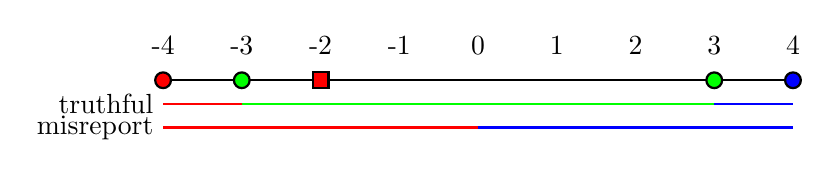
\begin{tikzpicture} [scale = 1] 
\draw[thick] (-4.0, 0.0) -- (4.0, 0.0);
\draw[fill = red, thick] (-4.0, 0.0) circle [radius = 0.1];
\draw[fill = red, thick] (-2.1, -0.1) rectangle (-1.9, 0.1);
\draw[fill = green, thick] (-3.0, 0.0) circle [radius = 0.1];
\draw[fill = green, thick] (3.0, 0.0) circle [radius = 0.1];
\draw[fill = blue, thick] (4.0, 0.0) circle [radius = 0.1];
\draw[red, thick] (-4.0, -0.3) -- (-3.0, -0.3);
\draw[green, thick] (-3.0, -0.3) -- (3.0, -0.3);
\draw[blue, thick] (3.0, -0.3) -- (4.0, -0.3);
\node[left] at (-4.0, -0.3){truthful};
\draw[red, thick] (-4.0, -0.6) -- (0.0, -0.6);
\draw[green, thick] (0.0, -0.6) -- (0.0, -0.6);
\draw[blue, thick] (0.0, -0.6) -- (4.0, -0.6);
\node[left] at (-4.0, -0.6){misreport};
\node[above] at (0.0, 0.2){$0$};
\node[above] at (1.0, 0.2){$1$};
\node[above] at (2.0, 0.2){$2$};
\node[above] at (3.0, 0.2){$3$};
\node[above] at (4.0, 0.2){$4$};
\node[above] at (-1.0, 0.2){-$1$};
\node[above] at (-2.0, 0.2){-$2$};
\node[above] at (-3.0, 0.2){-$3$};
\node[above] at (-4.0, 0.2){-$4$};
\end{tikzpicture} 
\end{figure}
\end{frame}

\begin{frame} \frametitle{Intuition}
\begin{itemize}
\item An agent in class $a $ is misclassified as $b $ may want to misreport as $c $ to move the decision boundary between $a $ and $b. $
\item Two conditions to prevent this incentive incompatibility problem:
\end{itemize}
\begin{enumerate}
\item Adding one class $a $ agent at $x $ moves the decision boundary between $a $ and $b $ away from $x $ (so that $x $ is relatively more likely to be classified as $a $).
\item Adding one class $c $ agent at $x $ does not change the decision boundary between $a $ and $b. $
\end{enumerate}

\end{frame}

\begin{frame} \frametitle{Formal Conditions}
\begin{itemize}
\item Monotonic condition (MC) and Independence of Irrelevant Alternatives condition (IIA), for any $x $ and $a , b, $
\end{itemize}
\begin{enumerate}
\item $\dfrac{\mathbb{P}\left\{Y = a | x, w^\star \left(S\right)\right\}}{\mathbb{P}\left\{Y = b | x, w^\star \left(S\right)\right\}} \leq  \dfrac{\mathbb{P}\left\{Y = a | x, w^\star \left(S \cup \left\{\left(x, y = a\right)\right\}\right)\right\}}{\mathbb{P}\left\{Y = b | x, w^\star \left(S \cup \left\{\left(x, y = a\right)\right\}\right)\right\}}.$
\item $\dfrac{\mathbb{P}\left\{Y = a | x, w^\star \left(S\right)\right\}}{\mathbb{P}\left\{Y = b | x, w^\star \left(S\right)\right\}} = \dfrac{\mathbb{P}\left\{Y = a | x, w^\star \left(S \cup \left\{\left(x', y' \notin \left\{a, b\right\}\right)\right\}\right)\right\}}{\mathbb{P}\left\{Y = b | x, w^\star \left(S \cup \left\{\left(x', y' \notin \left\{a, b\right\}\right)\right\}\right)\right\}}.$
\end{enumerate}

\end{frame}

\begin{frame} \frametitle{Outline of Proof}
\begin{itemize}
\item Let $w^\star $ be the estimated parameters when everyone reports truthfully and $w^{\dagger}$ be the estimated parameters when some agent $i $ misreports $y^{\dagger}_{i} \neq  y_{i.}$
\item Suppose for a contradiction that $\mathbb{P}\left\{Y = y_{i} | x_{i}, w^\star \right\} < \mathbb{P}\left\{Y = y_{i} | x_{i}, w^{\dagger}\right\}$.
\item MC and IIA implies $\mathbb{P}\left\{Y_{i} = y^{\dagger}_{i} | x_{i}, w^\star \right\} > \mathbb{P}\left\{Y = y_{i} | x_{i}, w^{\dagger}\right\}$.
\item Then, the optimality of $w^\star $ contradicts with the optimality of $w^{\dagger.}$
\end{itemize}
\end{frame}

\begin{frame} \frametitle{ERM Classifiers}
\begin{itemize}
\item MC and IIA may not be sufficient.
\item A normalization condition is required: the sum of the losses over all classes for any point must be constant.
\item ERM with zero-one loss satisfies MC and the normalization condition but does not always satisfy the IIA condition.
\end{itemize}
\end{frame}

\begin{frame} \frametitle{Separable Classifiers}
\begin{itemize}
\item If separate parameters are estimated for separate classes (independent of the points from other classes), then MC and IIA are always satisfied, therefore these classifiers are always IC.
\item Bayes classifiers with parameters estimated by maximum likelihood, including commonly used naive Bayes classifiers, are separable.
\item Mixture of Gaussian classifier is not separable.
\item The proof for kernel density estimators is similar.
\end{itemize}
\end{frame}

\begin{frame} \frametitle{Separable Logistic Regression}
\begin{itemize}
\item Multi-class logistic regression is not separable.
\item One-vs-one and one-vs-all logistic regressions are also not separable, but they are IC (because the binary classifiers are IC).
\end{itemize}
\end{frame}

\end{document}
